\chapter{Thermo-mechanical consolidation -- THM-Processes}
\label{sec:thm}

\section{Theory}
For thermo-mechanical consolidation, the vapor diffusion is considered.  The governing equations, which are
essential for the analysis, are detailed hereafter.
\subsection{Non isothermal flow in porous media}
Consider a general case of a flow problem in deformable porous media
under the Richard's approximation. With the classical Darcy's law,
the large scale water flow $\Fluxf$ is defined as
\begin{equation}
\Fluxf = -\poro \sat\left(\dens_w \dfrac{k_{rel}\per}{\mu}(\nabla
p-\dens\grv)\right)
 \label{eq:fflux}
\end{equation}
where $\sat$ is water saturation, $p$ is the water pressure,
$\dens$ is density, $n$ is effective porosity of the media, $\mu$ is
viscosity of flow, $k_{rel}$ is the relative permeability tensor,
$\grv$ is the gravity force by density  and $\per$ denotes
permeability. Meanwhile, we consider vapor flow  filled pores due to
molecular diffusion, which is coupled with temperature. Similar to
what is defined in \cite{Jonny05}, the vapor flow is given by
\begin{equation}
\Fluxv = -D_{pv}\nabla P-f_{Tv}D_{Tv}\nabla T
 \label{eq:fluxv}
\end{equation}
where ${f_Tv}$ is a thermal diffusion enhancement factor takes value
of 1.0 in the present simulation, $D_{pv}$ and $D_{Tv}$ are
diffusion coefficients takes form as
\begin{equation}
\begin{array}{lcl}
D_{pv}&=& \dfrac{D_v\dens_v}{\dens_wRT_{abs}}\\
D_{Tv}&=& D_v\left(h\pD{\dens_{\scriptscriptstyle vS}}{T}-\dfrac{\dens_v P}{\dens_w R T^2_{abs}}\right)\\
\end{array}
 \label{eq:diffus}
\end{equation}
with $h$, the relative humidity according to
\begin{equation}
h=e^{P/\dens_w R T_{abs}}
 \label{eq:hum}
\end{equation}
 $R=461.6J/kgK$, the specific gas constant for water vapour,
$\dens_{\scriptscriptstyle vS}$, the saturated vapour density given
by
\begin{equation}
\dens_{\scriptscriptstyle  vS}=10^{-3}\, e^{19.891-4975/T_{abs}}
 \label{eq:vap}
\end{equation}
and vapour density $\dens_v = h\, \dens_{\scriptscriptstyle vS}$.

 The expressions of flow defined in (\ref{eq:fflux}) and (\ref{eq:fluxv}) lead the
governing equation of flow field in the terms of mass balance
equation given by
\begin{gather}
\poro\left[\dfrac{\dens_w-\dens_v}{\dens_w}\pD{\sat}{\pres}+
\sat\beta_p+(1-\sat)\dfrac{\dens_v}{\dens^2_w R T_{abs}}   \right]
\pD{\pres }{t} \nonumber
\\
+  \nabla \cdot \left(\Fluxf+\Fluxv\right)/\dens_w+\sat
\frac{\partial}{\partial t}(\nabla\cdot \Disp) \nonumber
\\
\poro \dfrac{1-S}{\dens_w}\left(h \pD{\dens_{\scriptscriptstyle
vS}}{T} +\dfrac{\dens_v \pres}{R T^2_{abs}}  \right) \pD{T }{t} =0
  \label{eq:gv1}
\end{gather}
for any point $\Point\in \Omega\in \mathbb{R}^{\mathrm{n}}$ with
$\mathrm n$ the dimension of the real space. %%
In eqn. \ref{eq:gv1}, $\beta_p$ is the storitivity.  The unknown of
eqn. (\ref{eq:gv1}) to be solved are saturation of the phase
$\sat$, fluid pressure
 $p$ and the coupling term, i.e. temperature and displacement $\Disp$,
deduced by solid deformation.  The boundary conditions for this
problem can be simplified for this Richard's flow model
\begin{gather}
\Fluxf\cdot \nrl = q_{\scriptscriptstyle{\Gamma}}, \forall\,
\Point\,\in
\partial \Omega
 \label{eq:bcgv1}
\end{gather}
or Dirchlet type as
\begin{gather}
\pres = \pres_{\scriptscriptstyle{\Gamma}}, \quad \sat =
\sat_{\scriptscriptstyle{\Gamma}},
 \forall\, \Point\, \in \partial \Omega
 \label{eq:bcgv2}
\end{gather}
This initial-boundary-value-problem can be solved with the
corresponding initial condition of unknowns.
\subsection{Deformation}
Assuming solid grains itself are incompressible, i.e. $d^s\Disp/d^s
t = 0$, deformations in porous media can be described by the
momentum balance equation in the terms of stress as
\begin{equation}
\nabla \cdot (\Stress -\sat p\, \I -\alpha \I \Delta T) + \dens\grv
= 0 \label{eq:momb1}
\end{equation}
and  for bentonite material
\begin{equation}
\nabla \cdot (\Stress  -\alpha\, \I \Delta T) + \dens\grv = 0
\label{eq:momb2}
\end{equation}
and for rock,  where $\Stress$ is the effective stress of the porous
medium, $\alpha$ is the thermal expansion coefficient,  $\I$ is the
identity. Density of porous media consists of the portion
contributed by liquid $l$ and by the portion contributed of solid as
$\dens=\poro\dens^l+(1-\poro)\dens^s$.

The swelling pressure in bentonite is calculated by
\[
   \Stress_{sw}=\sat^2 \stress_{sw}^{max}\,\I
\].

\subsection{Heat transport}
For heat transport problem, we consider the convective transport,
i.e. the transport of heat by flow. There are two basic kinds of
convection recognized such as \emph{forced convection} and
\emph{free convection}. In the former, the velocity of convective
motion does not has any impact on the temperature on the fluids and
the heat energy transport is forced by the flow movement. In the
latter, flow velocities are driven solely by buoyancy effects in the
fluid, and these are related to temperature change through the
coefficient of thermal expansion. In real ground water systems,
there is a mixture of both types of convection. The simple
expression of heat flux in forced convection is given by
\begin{equation}
 \Flux_{\mbox{\tiny T}} = -K_e\nabla\,T+\poro\sum_{\gamma}^{phase}(\densc\HC^{\gamma}) T\vel
 \label{eq:tflux}
\end{equation}
where $K_e$ is the heat conductivity,
$\sum_{\gamma}^{phase}(\densc\HC^{\gamma}) T\vel$ is the flux of
heat transported by velocity $\vel$ per unit area, and across the
entire rock face this flux is reduced by the effective porosity,
$\poro$. With the definition of heat flux (\ref{eq:tflux}), the
governing  equation of the convective heat transport can be derived
for any point $\Point\in \Omega\in \mathbb{R}^{\mathrm{n}}$ as
\begin{equation}
 \sum_{\gamma}^{phase}(\densc\HC^{\gamma})\pD{T}{t}-\nabla \Flux_{\mbox{\tiny T}}+Q_{\mbox{\tiny T}}=0
 \label{eq:tgrn}
\end{equation}
with boundary condition
\begin{equation}
 \Flux_{\mbox{\tiny T}}\cdot\nrl=q_{\mbox{\tiny
 T}}\vert_{\scriptscriptstyle{\Gamma}},\, \mbox{or}\quad
 T=T_{\scriptscriptstyle{\Gamma}}, \,
 \forall\, \Point\, \in \partial \Omega
 \label{eq:tbc}
\end{equation}
and initial condition
\begin{equation}
 T(\Point)=T_0(\Point), \, \forall\, \Point\, \in \Omega
 \label{eq:tini}
\end{equation}

%------------------------------------------------------------------
\subsection[Repository in crystalline rock with unsat. bentonite buffer]{Repository in crystalline rock with unsaturated bentonite buffer: DECOVALEX Task IV - THM1}

\subsubsection*{Problem definition}
This example is dealing with fully coupled
thermo-hydraulic-mechanical (THM) processes in geotechnical
applications. This model is developed in the framework of Task D of
DECOVALEX III project (\texttt{www.decovalex.com}). This DECOVALEX test
case was designed by \cite{LBNL} for modeling THM coupling processed in FEBEX type nuclear waste repository.
Fig. \ref{fig_mod} illustrates the set-up of the model, in which, V1, $\cdots$, V6 indicate the observation points.
\begin{figure}[H]
  \centering
  \includegraphics[scale=0.6]{THM/set-up.eps}
  \caption{Model step-up (\cite{LBNL})}
  \label{fig_mod}
\end{figure}
A full scale simulation of this problem is given in \cite{WXNKHK:05}. The results are compared with that obtained
 by other research teams\cite{RBCKLOWZ:06}.  In order to save benchmark running time and keep the original physics of the problem,
     this benchmark takes a patch cut from the full domain and the results of
  the full scale simulation at the edge of the patch as boundary condition. The initial stress is obtained
     by excavation simulation. The simulation gives results of THM processes till 1000 years
    The domain contains that occupied by the waste canister, bentonite \mbox{buf\mbox{}fer} and surrounding rock. A triangular
      mesh of the domain is shown in Fig. \ref{fig:THMMesh}.
  \begin{figure}[!htb]
  \centering
   \includegraphics[scale=0.3]{THM/thm1_cut.eps}\\
  \caption{Near field of DECOVALEX THM1 model }
  \label{fig:THMMesh}
\end{figure}

The simulation is split in two phases. In the first phase, an initial state of stress, water pressure and temperature are established by excavation simulation. The operation simulation, that means the THM simulation after having installed the canister and bentonite, is done in a second phase.

The simulation of the excavation phase was done within 4 steps (Wang et al., 2007). At first the initial stress of the whole domain was calculated. Then the released force on the surface of the excavation tunnel was obtained. In a third step the domain with the excavation was analysed with the released force as unique boundary condition. The last step is the combination of step 1 and 3: the stress after excavation. After this the initial conditions of water pressure and temperature were calculated by simulating one time step of the TH coupled process. In the second phase the THM coupled processes in the bentonite and the near field rock mass on the base of the described initial condition set-up are modelled for a period of 1 million years under the assumption that the permeability of the rock mass and bentonite is constant. The initial and boundary conditions that are indicated in Fig. \ref{fig82} are relevant for the simulation run. To avoid flow within the canister domain the method of activating and deactivating elements was applied. Thus during the flow process the elements of the canister are devoid with a zero Neumann boundary condition on the surface of the canister. The heat power function which represents the source term of heat (due to radioactive decay, Fig. \ref{fig82}) in the canister was given in a graphical form to the simulation teams (Birkholzer et al., 2007).

\subsubsection*{Initial and Boundary conditions}
Values of variables at the cut interfaces of the full scale domain are taken as boundary condition directly
 (see Fig. \ref{fig:THMMesh} and cf.  \cite{WXNKHK:05} and \cite{RBCKLOWZ:06}).

\subsubsection*{Material properties}
The material parameters for rock mass and bentonite are given in
Table \ref{tab:thm_rock} and \ref{tab:thm_bentonite},
respectively.

\begin{table}[H]
\begin{center}
\begin{tabular}{lll}
\hline \hline
Parameter   &  Unit  & Value\\
\hline \hline
 Density &  $kg/m3$ &  2700 \\
\hline
 Young's modulus &  $GPa$ &  $35$ \\
\hline
 Poisson ratio & - &  0.3 \\
\hline
 Biot's constant & - &  1 \\
\hline
 Thermal expansion coefficient &  - &  $1.0
\times10^{-5}$ \\
\hline
 Thermal conductivity &  $W/mK$ &  3\\
\hline
 Thermal capacity &  $J/kgK$ &  900\\
\hline
 Porosity & - &  0.01 \\
\hline
 Saturated permeability &  $m2$  & $1.0
\times10^{-17}$ \\
\hline \hline
\end{tabular}
\end{center}
\caption{Rock Mass}
\label{tab:thm_rock}

\end{table}
%%%%%
\begin{table}[H]
\begin{center}
\begin{tabular}{lll}
\hline \hline
 Density &  $kg/m3$ &  1600 \\
\hline
 Young's modulus &  $MPa$ &  $317$\\
\hline
 Poisson ratio & - &  0.35 \\
\hline
 Biot's constant & - &  1 \\
\hline
Tortuosity &  - &  $0.8$ \\
\hline
 Porosity & - &  0.41 \\
\hline
 Thermal expansion coefficient &  - &  $1.0
\times10^{-5}$ \\
\hline
 Thermal conductivity &  $W/mK$ &  $c_s=1.38T+732.5$\\
\hline
 Thermal capacity &  $J/kgK$ &  $\kappa_m=1.28-\frac{0.71}{1+e^{10(S_w-0.65)}}$\\
\hline
 Saturated permeability &  $m2$  & $2.0
\times10^{-21}$ \\
\hline \hline
\end{tabular}
\end{center}
\caption{Bentonite}
\label{tab:thm_bentonite}
\end{table}

A time-depending heat power function is given in order to describe
the heat source condition of the containment. Measured
soil-water-characteristic curves are used in order to describe the
thermo-hydraulic behaviour. The dependency of capillary pressure
as well as relative permeability on liquid saturation for both of
rock and bentonite are depicted in Fig. \ref{fig:cp_rp}.
\begin{figure}[!htb]
  \begin{center}
    \begin{minipage}[t]{0.45\textwidth}
      \begin{center}
        \includegraphics[scale=0.3]{THM/capsat_new.eps}\\
        \centerline{Capillary pressure}
      \end{center}
    \end{minipage}
  %%\hspace{0.01\textwidth}
    \begin{minipage}[t]{0.45\textwidth}
      \begin{center}
        \includegraphics[scale=0.3]{THM/persat.eps}\\
        \centerline{Relative permeability}
      \end{center}
    \end{minipage}\\
  \end{center}
  \caption{Capillary pressure - relative permeability - functions}
  \label{fig:cp_rp}
\end{figure}

\subsubsection*{Results}

Evaluation method: The numerical results are compared to those of the simulation programmes TOUGH-FLAC (TH processes coupled in TOUGH; M-processes with FLAC) and ROCMAS (THM processes coupled) (Birkholzer et al., 2007).

Fig. \ref{fig_THMdTS} provides the distribution of temperature and saturation after 1 year.
\begin{figure}[H]
  \begin{center}
  \epsfig{figure=THM/d_T_1y.eps,height=5cm}
  \epsfig{figure=THM/d_sat_1y.eps,height=5cm}
  \end{center}
  \caption{Distribution of temperature and saturation}
  \label{fig_THMdTS}
\end{figure}
%%
Fig. \ref{fig_THMdSV} provides the distribution of vertical stress and fluid velocity after 1 year.
\begin{figure}[H]
  \begin{center}
  \epsfig{figure=THM/d_syy_1y.eps,height=5cm}
  \epsfig{figure=THM/d_vel_1y.eps,height=5cm}
  \end{center}
  \caption{Distribution of vertical stress and fluid velocity}
  \label{fig_THMdSV}
\end{figure}
Fig. \ref{fig_THMvts_t} shows the evolution of temperature and saturation at observation points.
\begin{figure}[H]
  \begin{center}
  \epsfig{figure=THM/d_v_T_t.eps,height=5cm}
  \epsfig{figure=THM/d_v_sat_t.eps,height=5cm}
  \end{center}
  \caption{Evolution of temperature and saturation}
  \label{fig_THMvts_t}
\end{figure}
Fig. \ref{fig_THMvsu_t} shows the evolution of horizontal stress and vertical displacement at observation points.
\begin{figure}[H]
  \begin{center}
  \epsfig{figure=THM/d_v_sxx_t.eps,height=5cm}
  \epsfig{figure=THM/d_v_uy_t.eps,height=5cm}
  \end{center}
  \caption{Evolution of horizontal stress and vertical displacement}
  \label{fig_THMvsu_t}
\end{figure}
Fig. \ref{fig_THMvel} gives vertical velocity profile along horizontal line cross the canister center.
\begin{figure}[H]
  \begin{center}
  \epsfig{figure=THM/h_vel.eps,height=5cm}
  \end{center}
  \caption{Vertical velocity profile}
  \label{fig_THMvel}
\end{figure}
The above results agree with that obtain by using a full domain.

\subsubsection*{Benchmark deposit}
\begin{tabular}{|l|l|l|}
  \hline
  Benchmark & Problem type & Path in benchmark deposit \\
  \hline
 \emph{thm\_decov}& THM & benchmarks\verb \THM\ \\
  \hline
\end{tabular}
%%%%%%%%%%%%%%%%%


%\section{Thermo-poro-plasticity}
%
%\subsection{Saturated thermo-poro-plastic plate (2D)}
%
%\begin{description}
%  \item[Benchmark name:] \emph{thm\_quad}.
%\end{description}
%
%\subsection{Unsaturated thermo-poro-plastic plate (2D)}
